\subsection{Overview}
The system paradigm is client-server. In particular, there is a thin client and a fat server. 
The client contains only a presentation layer. 
The server, instead, contains both the business application logic and the data management logic. 
The system paradigm is client-server. In particular, there is a thin client and a fat server. The client contains only a presentation layer. The server, instead, contains both the business application logic and the data management logic. 
The layer of the application are:
\begin{itemize}
    \item \textbf{Presentation Layer:} it manages the presentation logic and all the interactions with the user.
    \item \textbf{Application Layer:} it manages all the functionalities of the system.
    \item \textbf{Data Layer:} it manages the access and the storage of data.
\end{itemize}

\begin{figure}[H]
    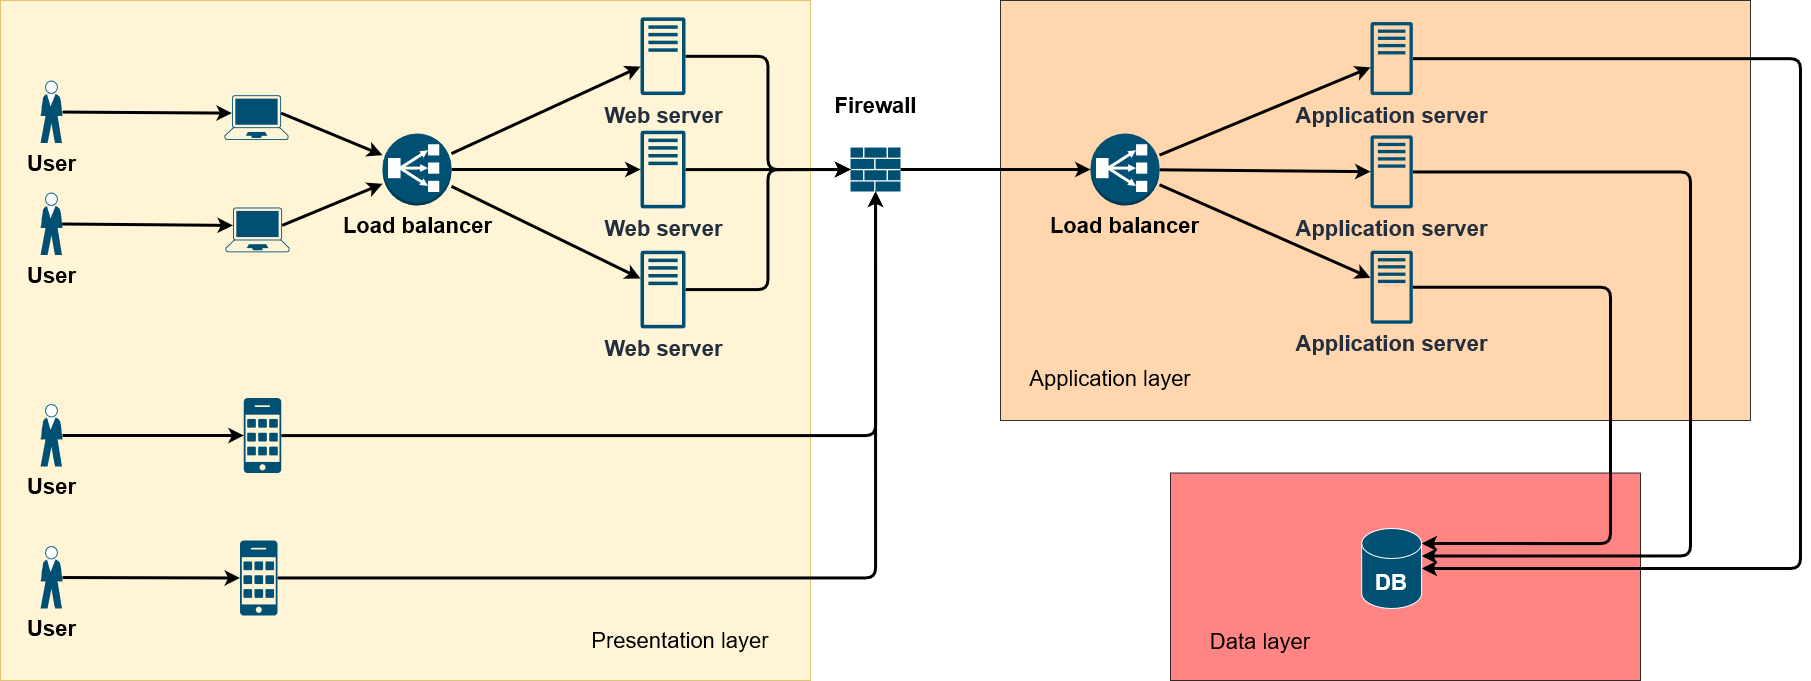
\includegraphics[width=\textwidth,height=\textheight,keepaspectratio]{Images/architectureDesignDiagram.png}
    \caption{Architecture of the application}
    \label{fig:architectue_diagram}
\end{figure}

As shown in figure \ref{fig:architectue_diagram} the application is divided into 3 layers and 4 tiers. Users can access the service
both from a mobile app or web interface. The figure shows the division of the different layers. Since the application follows the 
REST standard the servers are stateless. There will be a more precise description of the components in the following sections.

\subsection{Component View}
\begin{figure}[H]
    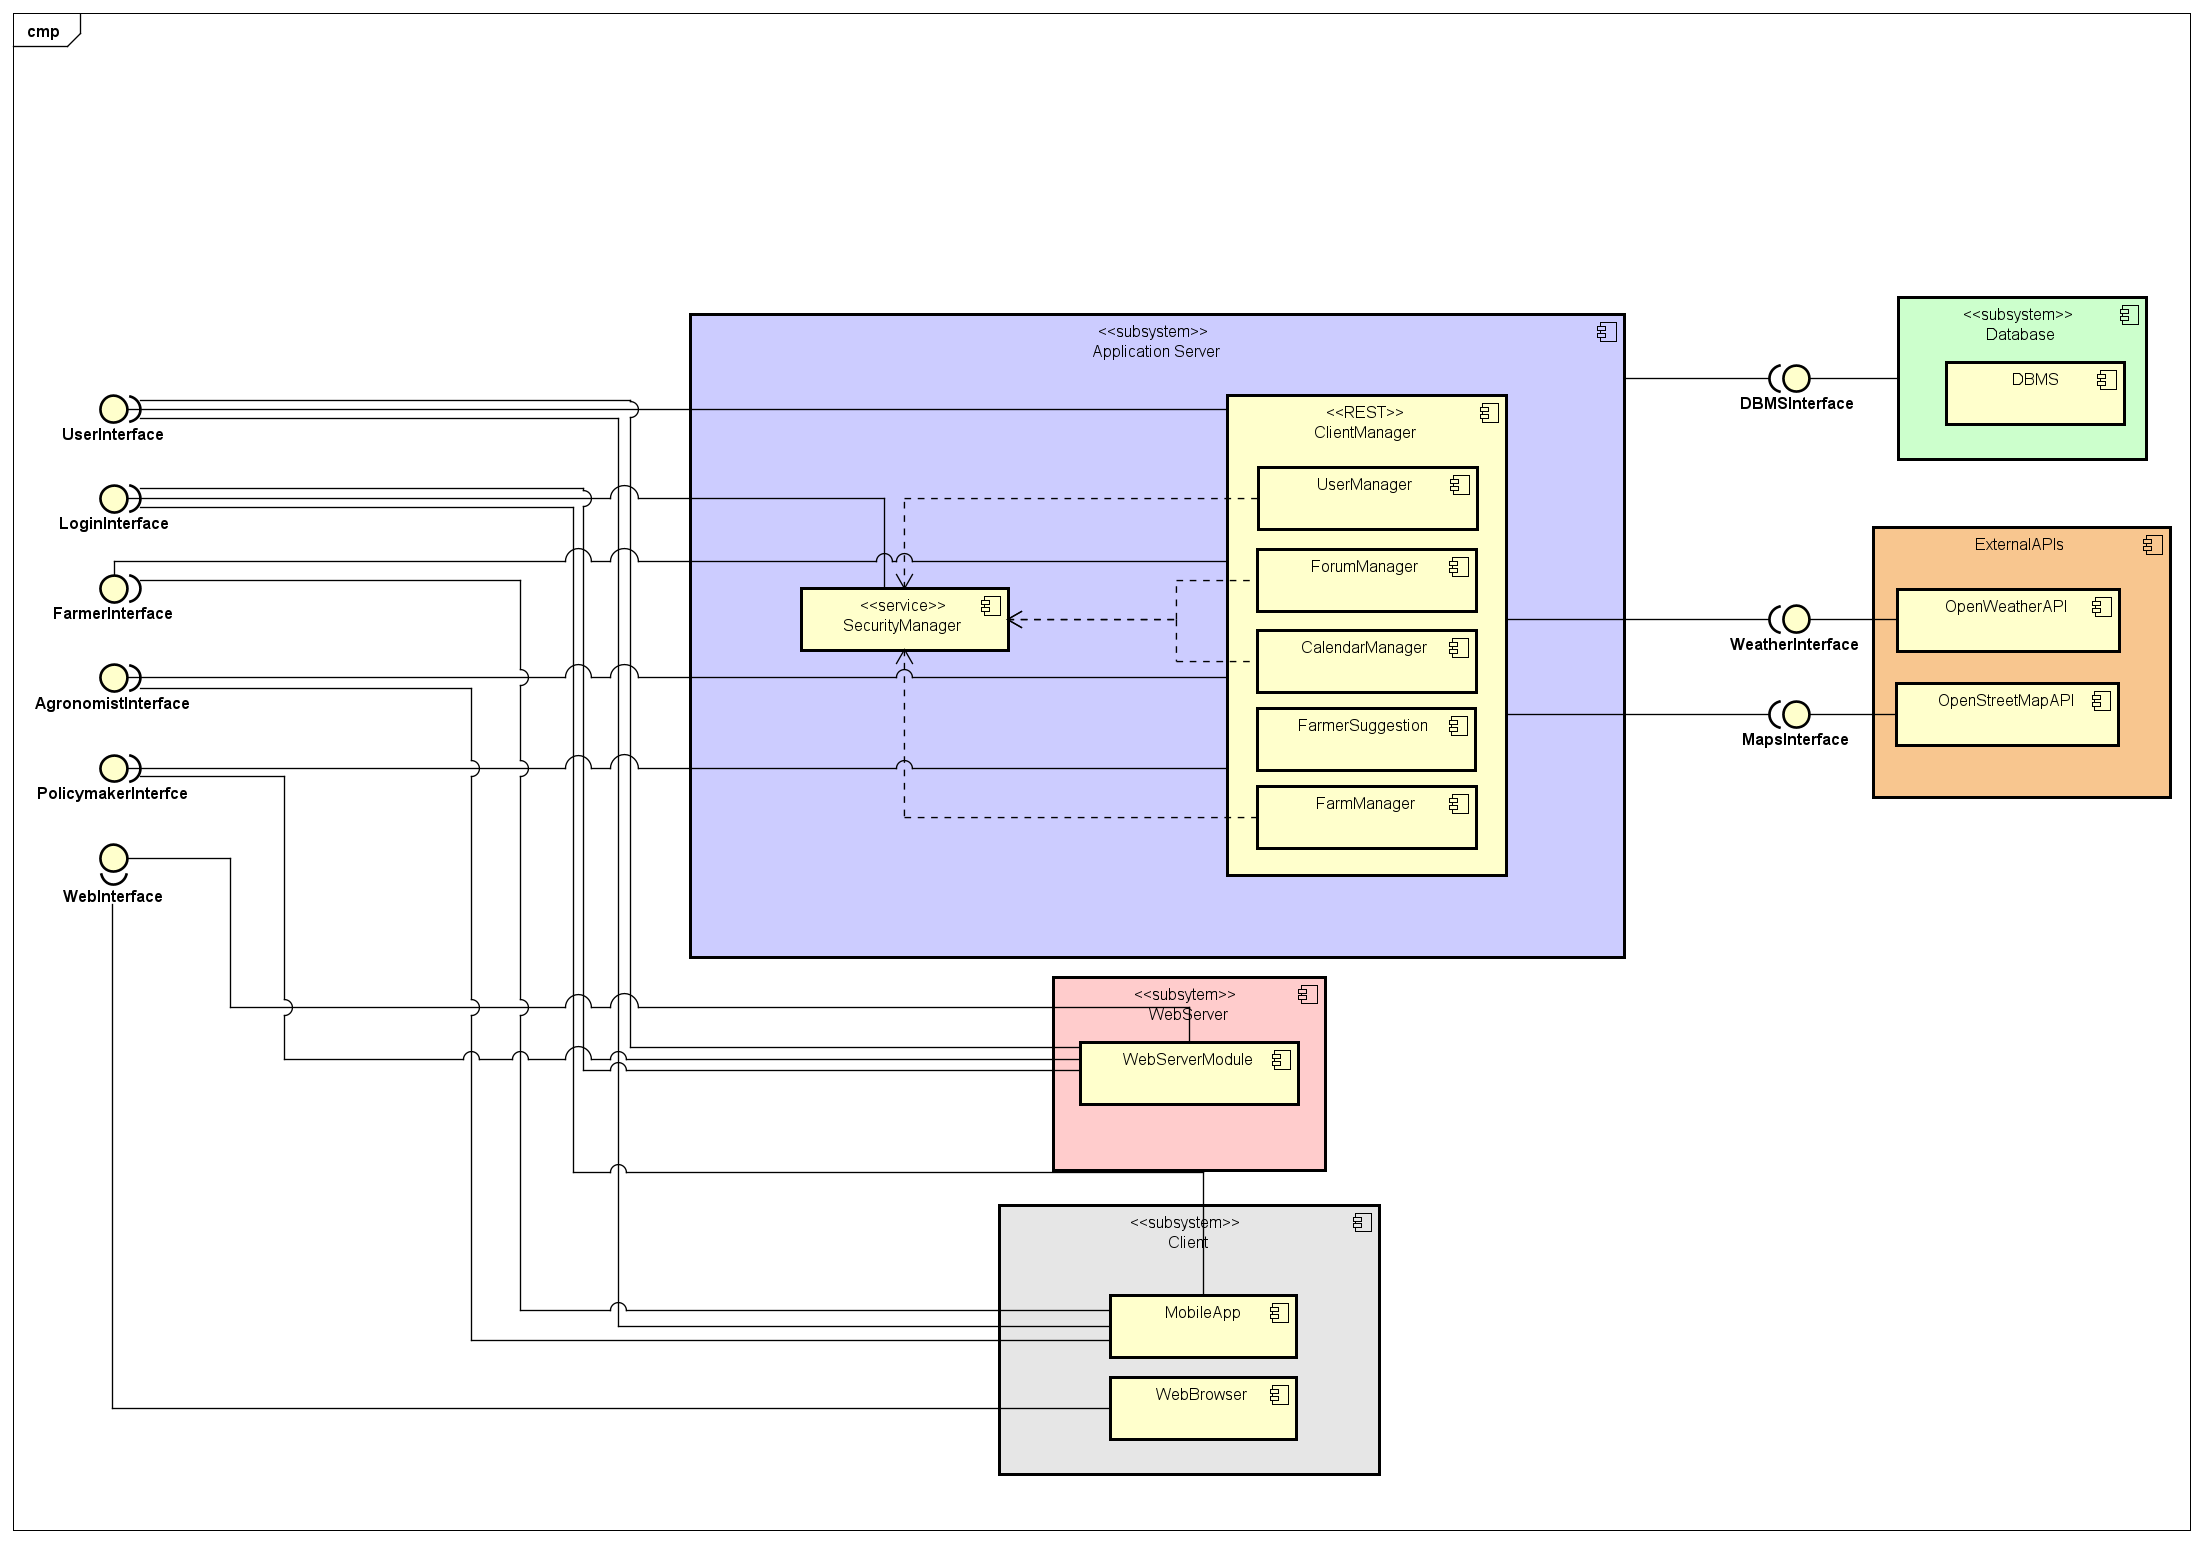
\includegraphics[width=\textwidth,height=\textheight,keepaspectratio]{Images/ComponentDiagram.png}
    \caption{Component Diagram}
    \label{fig:component_diagram}
\end{figure}

Figure \ref{fig:component_diagram}  represents in detail the layers described before. The web server has the function to
route the browser requests to the application server and send back its responses.

\begin{itemize}
    \item \textbf{Client Manager}\\
        This module handles all the requests made by the client. In the beginning,
        when the client is not logged in, the module offers (through
        the user manager) a loginInterface that allows the client to register and log in. After the login the module
        provide an interface based on the role of the user: FarmInterface for the farmer, AgronomistInterface for the agronomist,
        PolicymakerInterface for the policymaker.

    \item \textbf{User Manager}\\
        This module provides all the functionalities needed to manage the user. It includes signup and login as well as role checking 
        operation and information retrieving.
           
    \item \textbf{Forum Manager}\\
        This module provides all the functionalities through the ForumInterface for managing and using the forum. 
        It includes operations for creating and replying to a discussion on the forum.

    \item \textbf{Calendar Manager}\\
        This Module provides all the functionalities needed for the Agronomist to manage his calendar. In particular, it provides
        through, the AgronomistInterface, the possibility to add or remove an appointment, to confirm the daily plan and to check
        that each farm has at least two visits per year.

    \item \textbf{Farmer Suggestion}\\
        This module handles the creation and delivery of personalized suggestions to the Farmer. 

    \item \textbf{Farm Manager}\\
        This module provides to the Farmer all the functionalities for giving information about their farm. 
        It provides the possibility to add information about the harvest and to request help from the Agronomist.

    \item \textbf{Security Manager}\\
        This module handles all the security issues.
\end{itemize}

\newpage
\subsection{Deployment diagram}
\begin{figure}[H]
    \begin{center}
        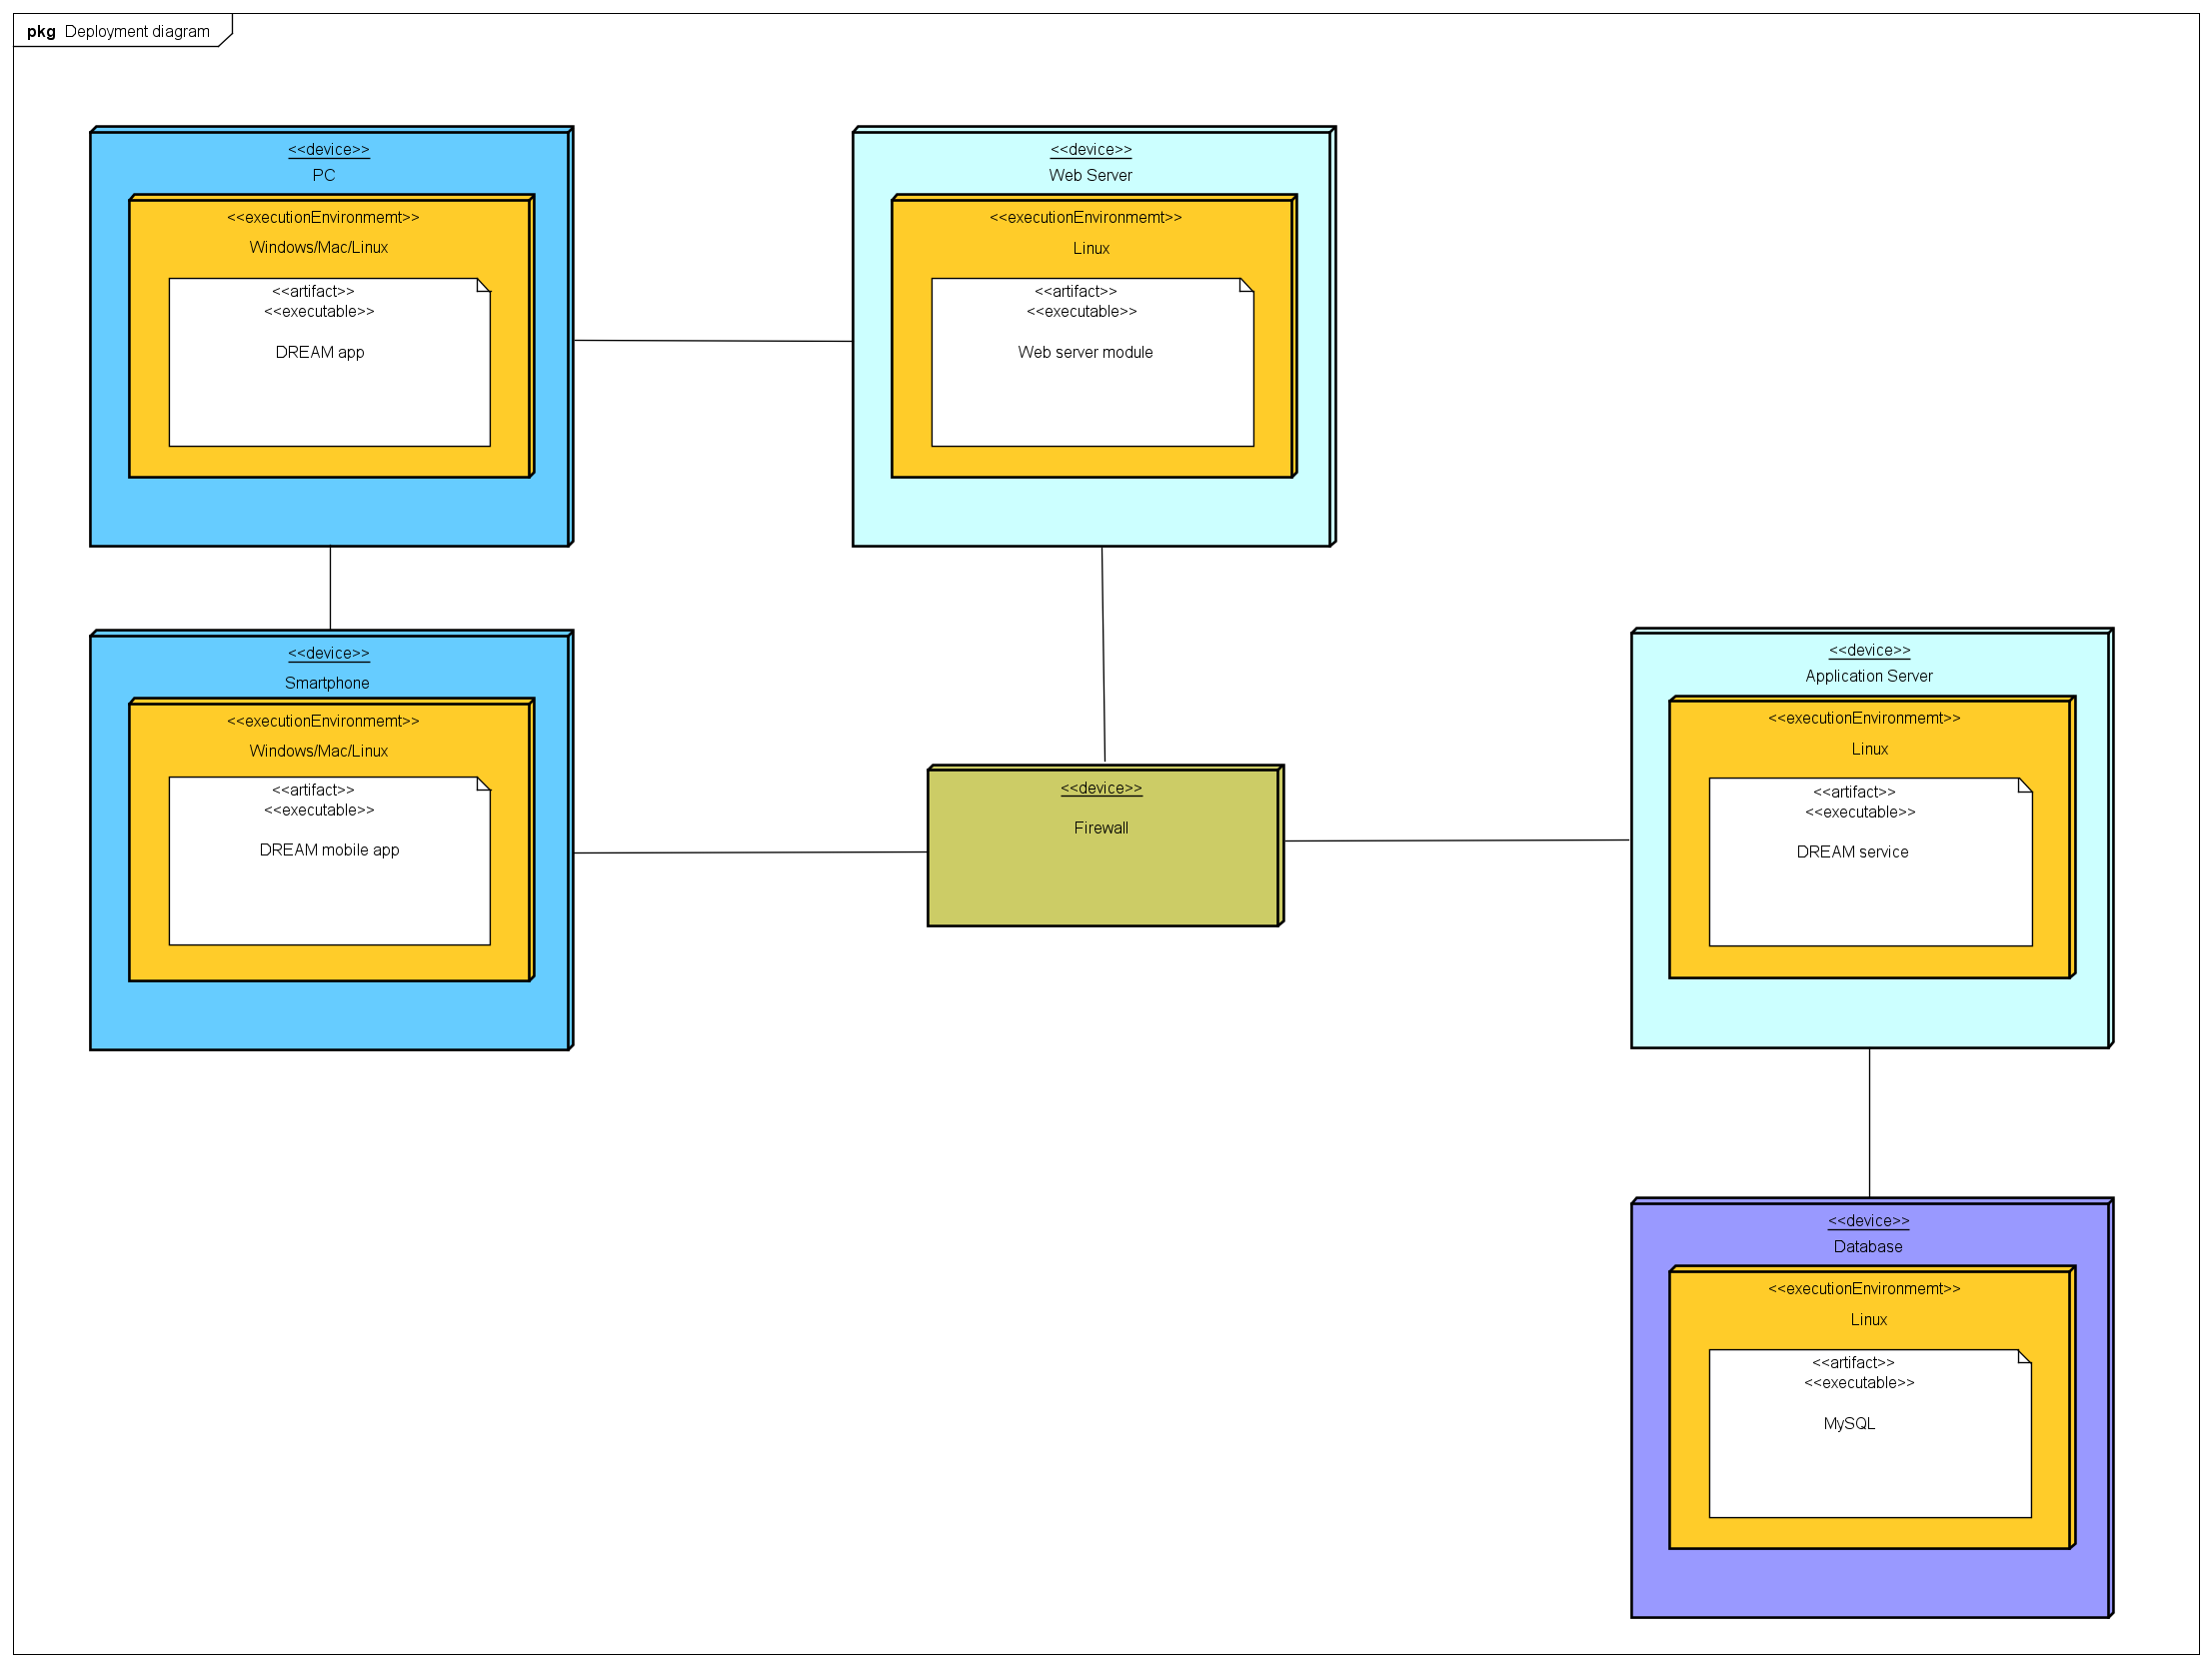
\includegraphics[width=\textwidth]{Images/DeploymentDiagram.png}
        \caption{Deployment Diagram}
    \end{center}
\end{figure}

The deployment diagram in figure shows the needed components for correct system behavior.
Each device owns its Operating System where the software runs. Firewall ensures application security.
\newline The tiers in the image are the following:
\begin{itemize}
    \item \textbf{Tier 1:} it is the client machine, which can be a computer with a web browser or the mobile
    application.
    \item \textbf{Tier 2:} includes the replicated web servers, which do not execute any business logic, but simply receive
    requests from the client, route them to the application servers and serve an HTML back to the client.
    \item \textbf{Tier 3:} it includes the application servers that contain the whole application layer and communicate to the data tier.
    \item \textbf{Tier 4:} it contains the DBMS servers that store and manage data, according to the instructions given by the application servers.
\end{itemize}

\newpage

\subsection{Component Interfaces}
\begin{figure}[H]
    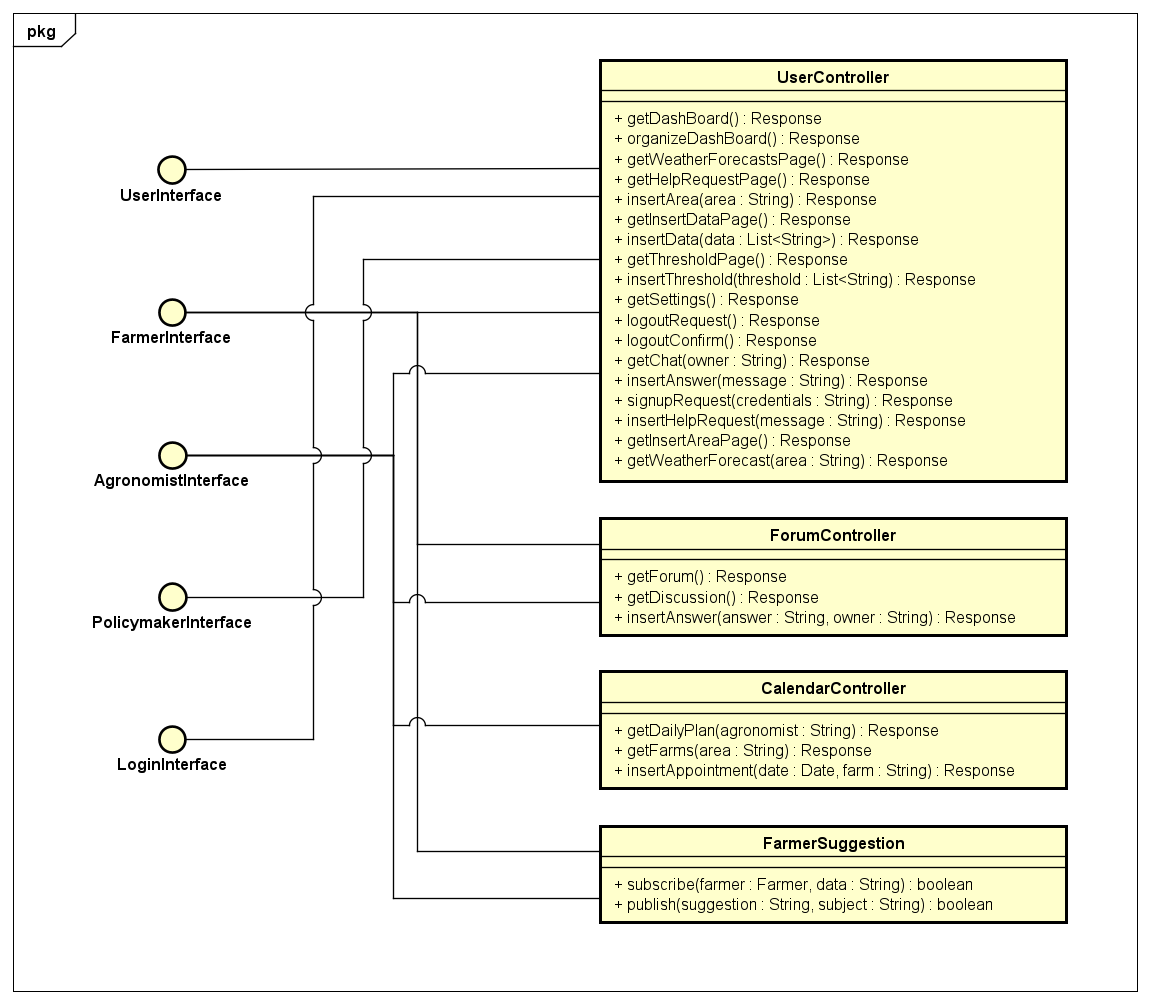
\includegraphics[width=\textwidth,height=\textheight,keepaspectratio]{Images/InterfaceDiagram.png}
    \caption{Interface Diagram}
    \label{fig:interface_diagram}
\end{figure}
Figure \ref{fig:interface_diagram} shows the main interfaces of the system.\newline
The \textbf{UserInterface} provides the functionalities common to all users, it is realized through just one controller the \textbf{UserController}. \newline
The \textbf{FarmerInterface} provides all the specific functionalities of the farmer and it is realized through three controllers: \textbf{UserController}, \textbf{ForumController}, \textbf{FarmerSuggestion}.\newline
The \textbf{AgronomistInterface} provides all the specific functionalities of the agronomist and it is realized through four controllers     :
\textbf{UserController}, \textbf{ForumController}, \textbf{FarmerSuggestion},\textbf{CalendarController}.\newline
The \textbf{PolicymakerInterface} provides all the specific functionalities of the policymaker and it is realized through one controller:
\textbf{UserController}.\newline
The \textbf{LoginInterface} provides all the functionalities for login and signup and it is realized through \textbf{UserController}.


\subsection{Logical Description of Data}
\begin{figure}[H]
    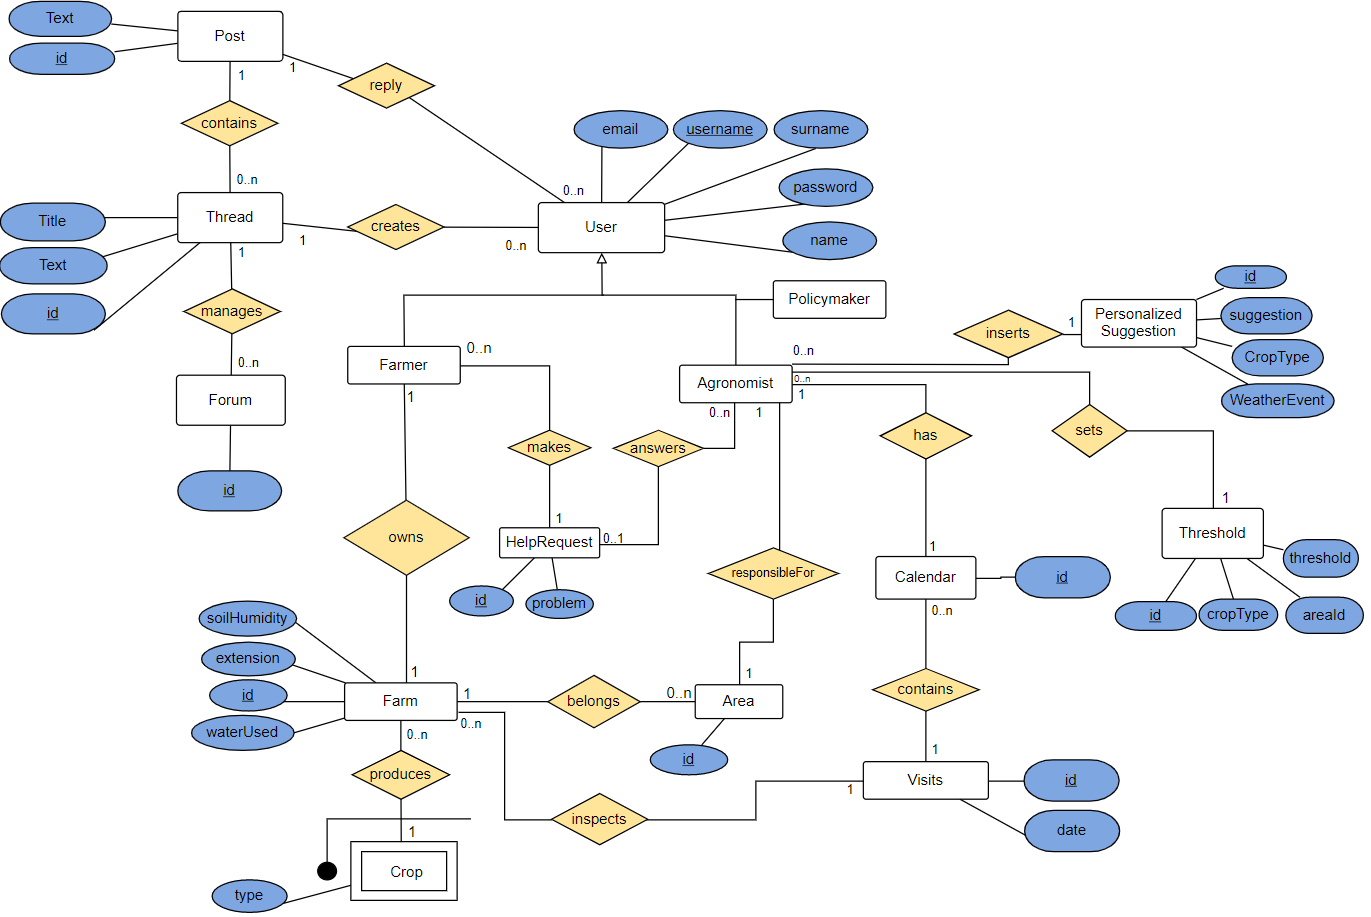
\includegraphics[width=\textwidth,height=\textheight,keepaspectratio]{Images/erDiagram.png}
    \caption{ER Diagram}
    \label{fig:er_diagram}
\end{figure}
Figure \ref{fig:er_diagram} shows a logical representation of the data that will be stored in the database of the system.
